\documentclass[14pt, fleqn, xcolor={dvipsnames, table}]{beamer}
\usepackage[T2A]{fontenc}
\usepackage[utf8]{inputenc}
\usepackage[english,russian]{babel}
\usepackage{amssymb,amsfonts,amsmath,mathtext}
\usepackage{cite,enumerate,float,indentfirst}
\usepackage{cancel}

\usepackage{tikz}                   
\usetikzlibrary{shadows}

% \usepackage{enumitem}
% \setitemize{label=\usebeamerfont*{itemize item}%
%   \usebeamercolor[fg]{itemize item}
%   \usebeamertemplate{itemize item}}

\graphicspath{{images/}}

\usetheme{Madrid}
\usecolortheme{seahorse}
\renewcommand{\CancelColor}{\color{red}}

\setbeamercolor{footline}{fg=Blue!50}
\setbeamertemplate{footline}{
  \leavevmode%
  \hbox{%
  \begin{beamercolorbox}[wd=.333333\paperwidth,ht=2.25ex,dp=1ex,center]{}%
    И. Кураленок, Н. Поваров, Яндекс
  \end{beamercolorbox}%
  \begin{beamercolorbox}[wd=.333333\paperwidth,ht=2.25ex,dp=1ex,center]{}%
    Санкт-Петербург, 2013
  \end{beamercolorbox}%
  \begin{beamercolorbox}[wd=.333333\paperwidth,ht=2.25ex,dp=1ex,right]{}%
  Стр. \insertframenumber{} из \inserttotalframenumber \hspace*{2ex}
  \end{beamercolorbox}}%
  \vskip0pt%
}
\newcommand\indentdisplays[1]{%
     \everydisplay{\addtolength\displayindent{#1}%
     \addtolength\displaywidth{-#1}}}
\newcommand{\itemi}{\item[\checkmark]}

\title{Переборные методы: сэмплирование\\\small{}}
\author[]{\small{%
И.~Куралёнок,
Н.~Поваров}}
\date{}

\begin{document}

\begin{frame}
\maketitle
\small
\begin{center}
\vspace{-60pt}
\normalsize {\color{red}Я}ндекс \\
\vspace{80pt}
\footnotesize СПб, 2013
\end{center}
\end{frame}

\section{Содержание}
\begin{frame}{Содержание}
\begin{enumerate}
  \item Понятие сэмплирования
  \begin{itemize}
   \item Процесс сэмплирования
   \item Основные методы сэмплирования
  \end{itemize}
  \item Переборные методы в ML
  \begin{itemize}
   \item Полный перебор
  \end{itemize}
  \item Hill climbing
  \item Сэмплирование марковскими цепями
  \begin{itemize}
   \item Metropolis-Hastings алгоритм
   \item Алгоритм Гиббса
  \end{itemize}
  \item Построение вероятностного пространства для максимизации
\end{enumerate}
\end{frame}

\begin{frame}{Понятие сэмплирования}
\textit{Сэмплирование} --- метод исследования множества путём анализа его подмножеств. \\
Применяется когда:
\begin{itemize}
   \item множество слишком велико для перебора;
   \item каждое дополнительное измерение дорого;
   \item предварительный анализ.
\end{itemize}
\end{frame}

\begin{frame}{Алгоритм сэмплирования}
\begin{enumerate}
   \item Понять какое множество мы изучаем
   \item Осознать что из этого множества мы можем измерить
   \item Определить количество измерений
   \item Разработать план сэмплирования
   \item Провести сэмплирование
\end{enumerate}
\end{frame}

\begin{frame}{Типы сэмплирования}
\begin{itemize}
   \item Вероятностное сэмплирование: 
   $$
   p(x),\forall x:p(x) > 0
   $$
   \textit{Например: попробуем посчитать соотношение мужчин/женщин}
   \item Невероятностное сэмплирование:
   $$
   p(x), \exists x: p(x) = 0
   $$
   \textit{Например: ``по результатам опроса superjob.ru, 100\% россиян пользуются интернетом''}
   \item Без возвращений
   \item С возвращениями
\end{itemize}
\end{frame}

\begin{frame}{Виды сэмплирования}
\begin{itemize}
   \item Вероятностное сэмплирование
   \begin{itemize}
    \item Простое вероятностное
    \item Систематическое
    \item Стратифицированное
    \item Пропорциональное
    \item Кластерное
   \end{itemize}
   \item Невероятностное сэмплирование
   \begin{itemize}
    \item Опрос ближайших
    \item Панельное сэмплирование
   \end{itemize}
\end{itemize}
\end{frame}


\begin{frame}{Как выбрать нужное?}
Надо учитывать:
\begin{itemize}
   \item природа и размер возможного сэмпла;
   \item наличие дополнительной информации об элементах;
   \item необходимя точность измерений;
   \item точность отдельных измерений в сэмплировании;
   \item стоимость измерений.
\end{itemize}
\end{frame}

\begin{frame}{Возвращаясь к ML}
$$
F_0 = \arg\max_F p(F|X)
$$
\begin{description}
  \item[\color{green}+] если известны вероятности можно попробовать посэмплировать решения;
  \item[\color{red}---] не определено пространство F;
  \item[\color{red}---] неясно как устроить обход.
\end{description}
\end{frame}

\begin{frame}{Иногда все просто}
$$
F_0 = \arg\max_{F \in \{f_i\}_{i=1}^n} p(F|X)
$$
\begin{enumerate}
  \item введём порядок обхода;
  \item переберём все возможные решения;
  \item составим взвешенное решение/выберем лучшее.
\end{enumerate}
\end{frame}

\begin{frame}{Но чаще всё непросто}
$$
F_0 = \arg\max_{F \in \{f_i\}_{i=1}^\infty} p(F|X)
$$
\begin{enumerate}
  \item введём порядок обхода;
  \item применим систематическое сэмплирование;
  \item составим взвешенное решение/выберем лучшее.
\end{enumerate}
\end{frame}

\begin{frame}{Случайное блуждание I}
Чтобы построить порядок обхода можно воспользоваться такой схемой:

$$\begin{array}{l}
F = F(x, \lambda), \lambda \in \mathbb{R}^n \\
F_t = F(x, \lambda_t) \\
\lambda_{t+1} = \lambda_t + \xi~~~~C(\lambda_{t+1} | \{\lambda_i\}_0^t) \\
\end{array}$$

\begin{itemize}
  \item будем блуждать по пространству параметров;
  \item необходимо определить:
  \begin{enumerate}
    \item способ сделать шаг;
    \item условие принятия этого шага.
  \end{enumerate}
\end{itemize}
\end{frame}

\begin{frame}{Случайное блуждание II}
На что стоит обратить внимание при построении блуждания:
\begin{itemize}
  \item размерность $\lambda$ может быть меньше чем кажется;
  \item ограничения на $\lambda$ существенно осложняют процедуру.
\end{itemize}
\end{frame}


\begin{frame}{Некоторые виды случайного блуждания}
\begin{itemize}
  \item множество фиксированных шагов $\xi \sim U(\{\xi_i\}_1^m)$;
  \item гауссовское $\xi_t \sim N(\mu, \sigma^2)$;
  \item самозависимое;
  \item etc.
\end{itemize}
\end{frame}

\begin{frame}{Simple hill climbing}
$$\begin{array}{l}
\xi \sim U(\{\xi_i\}_1^2n), \xi_{i\frac{i}{2}} = -1^{i mod 2}\omega, \xi_{ij} = 0, j \neq \frac{i/2},\\
\\
C(\lambda_{t+1}|\lambda_t) = \frac{p(F(\lambda_{t+1})|X)}{p(F(\lambda_t)|X)} > 1 \\
\end{array}$$
Свойства:
\begin{itemize}
  \item простой;
  \item быстро сходится;
  \item зависим от выбора начальной точки.
  \item etc.
\end{itemize}
\end{frame}

\begin{frame}{Random-restart (shotgun) hill climbing}
\begin{center}
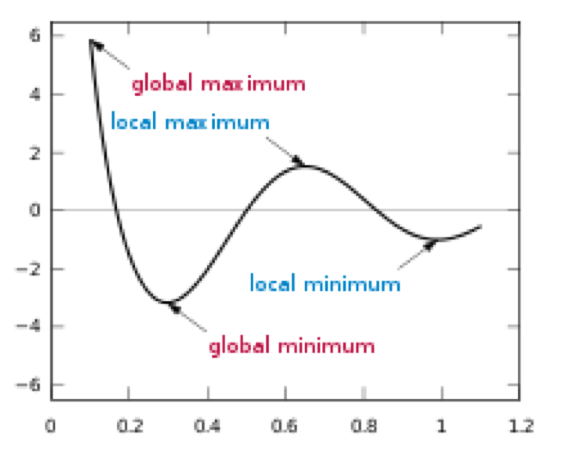
\includegraphics[width=0.4\textwidth]{hill_climb.png}
\end{center}
\footnotesize
Проблемы:
\begin{itemize}
  \item сходится в локальный максимум;
  \item может долго сходиться, если начало далеко от максимума;
  \item аллеи.
\end{itemize}
$\Rightarrow$ Можно рестартить hill climbing из разных начальных точек
\end{frame}

\begin{frame}{Интуиция}
Мы бы хотели получить сэмплирование, а для этого:
\begin{itemize}
  \item хорошо бы обойти всё пространство;
  \item нельзя всегда ходить ''по шерсти'';
  \item скорость движения должна меняться в зависимости от плотности.
\end{itemize}
$\Rightarrow$ Markov Chain Monte-Carlo (MCMC)
\end{frame}

\begin{frame}{Metropolis-Hastings алгоритм}

Введем $p(\lambda_1|\lambda_2)$, отвечающую за локальность.
$$\begin{array}{l}
\alpha = \frac{p(F_{\lambda_{t+1}}|X)p(\lambda_{t+1}|\lambda_t)}{p(F_{\lambda_t}|X)p(\lambda_t|\lambda_{t+1})}\\
\\
\psi \sim U(0,1)\\
\\
C(\lambda_{t+1}|\lambda_t) = \left\{  
           \begin{array}{ll}  
            1,& \alpha \ge \psi \\  
            0 &\\  
           \end{array}   
           \right.  
\end{array}$$
Например, $p(\lambda_{t+1}|\lambda_t) \sim N(\lambda_t,\sigma^2E)$ \\
Если $p(\lambda_1 | \lambda_2) = p(\lambda_2 | \lambda_1)$ --- это Metropolis \\ 
\end{frame}

\begin{frame}{Свойства}
\begin{center}
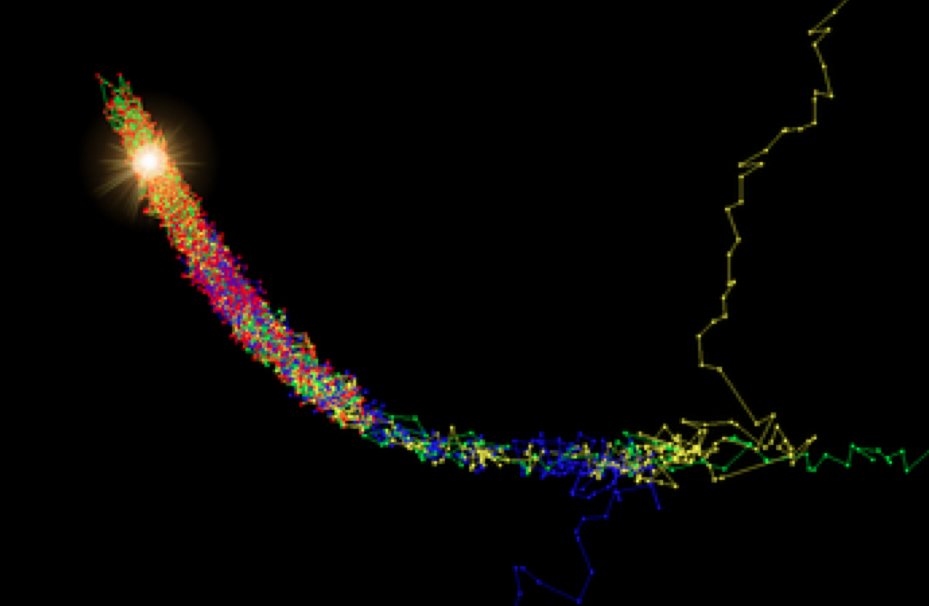
\includegraphics[width=0.5\textwidth]{mcmc.png}
\end{center}
\footnotesize
\begin{description}
  \item[\color{green}+] Обходит всё пространство
  \item[\color{green}+] Это действительно взвешенное сэмплирование
  \item[\color{red}---] Последовательные самплы похожи друг на друга
  \item[\color{red}---] На этапе разогрева показывает что-то странное
\end{description}
$\Rightarrow$ \textit{Точно придём в максимум!} \\
\end{frame}

\begin{frame}{Свойства}
\begin{center}
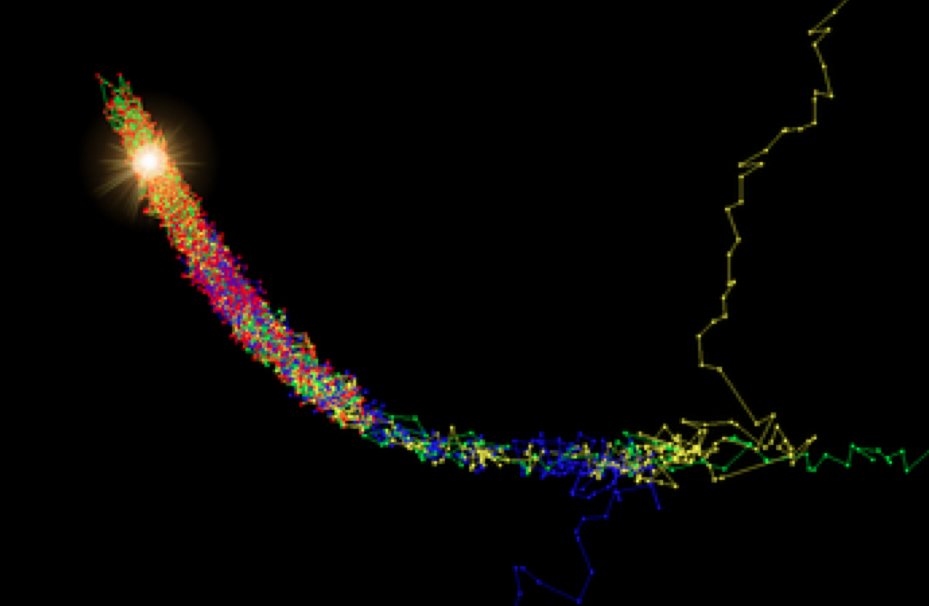
\includegraphics[width=0.5\textwidth]{mcmc.png}
\end{center}
\footnotesize
\begin{description}
  \item[\color{green}+] Обходит всё пространство
  \item[\color{green}+] Это действительно взвешенное сэмплирование
  \item[\color{red}---] Последовательные самплы похожи друг на друга
  \item[\color{red}---] На этапе разогрева показывает что-то странное
\end{description}
$\Rightarrow$ \textit{Точно придём в максимум!} \\
\textbf{Проблема только с тем, что придём за бесконечное время}
\end{frame}

\begin{frame}{Сложности в использовании}
\begin{itemize}
  \item Сходимость зависит от выбора $p(\lambda_{t+1}|\lambda_{t})$
  \item Если хотим использовать разумное распределение, оно многомерное $\Rightarrow$ его сложно реализовывать
\end{itemize}
\end{frame}

\begin{frame}{Пример с дартс I}
\small
Вася и Петя повесели на стене мишень и поиграли в дартс. На следующий день пришел их бригадир Юра и задался вопросом кто из подчиненных будет заделывать дырки в стенах.
\begin{itemize}
  \item Будет честнее, чтобы ``косой'' платил больше
  \item Дырки все одинаковые
  \item Каждый говорит: ``да я токо разок кинул!''
  \item Один признался, что: ``ну вот это --- моя дырка''
  \item Играли без употребления, так что можно считать, что кидали $\sim N(m_i, \Sigma_i), i \in$ \{Вася, Петя\} и параметры не менялись во времени
\end{itemize}
\textbf{Надо помочь Юре!}
\end{frame}

\begin{frame}{Пример с дартс II}
\small
При фиксированных параметрах вероятность увидить дырки $\{x_j\}, x_j \in \mathbb{R}^2$
$$
LL = \sum_j \log(\pi N(m_A, \Sigma_A)(x_j) + (1 - \pi) N(m_B, \Sigma_B)(x_j))
$$
где $A$ --- Вася, $B$ --- Петя, $\pi$ --- доля Васиных бросков, $m_i$ --- сбитость прицела, $\Sigma_i$ --- разброс стрелка. \\
Максимизировать такое добро трудновато из-за суммы под логарифмом. Было бы классно точно знать, что тот или иной бросок точно сделал Вася $A_t \in \{0,1\}$:
$$
LL = \sum_t A_t \log(N(m_A, \Sigma_A)(x_j)) +  (1 - A_t) \log(N(m_B, \Sigma_B)(x_j))
$$
В таком варианте все совсем просто считается (если мы еще не забыли формулу плотности нормального многомерного распределения :))
\end{frame}

\begin{frame}{Пример с дартс III}
\small
Если чуть более формально, то мы ввели скрытую/ненаблюдаемую переменную $I(A)$ (такое называется data augmentation) и хотим:
\begin{enumerate}
  \item Прикинуть начальные $m_i, \Sigma_i, \pi$
  \item Посчитать ожидание скрытого параметра $A_j = \mu({(m_i, \Sigma_i}, \pi)$
  \item В условиях найденных $A_j$ максимизировать $LL$
  \item Перейти к второму шагу до сходимости
\end{enumerate}
\end{frame}

\begin{frame}{Expectation maximization алгоритм}
\small
Фокус, который мы проделали называется $EM$-алгоритм. Пускай данные у нас состоят из видимой части $L$ и скрытой $Z$, $X = (L,Z)$. Мы хотим найти оптимальные параметры $\lambda$:
$$
LL(p(L|\lambda)) = LL(p(X|\lambda))
$$
\begin{enumerate}
  \item Возьмем какой-то $\lambda_0$
  \item Посчитаем ожидание (expectation step):
  $$
  E(\lambda | \lambda_t) = \mu\left(LL(\lambda,X) | Z,\lambda_t \right)
  $$
  \item Проведем оптимизацию (maximization step):
  $$
  \lambda_{t+1} = \arg \max_{\lambda} E(\lambda | \lambda_t)
  $$
  \item Перейти к второму шагу до сходимости
\end{enumerate}
\end{frame}

\begin{frame}{Алгоритм Гиббса}
В Метрополисе есть проблема: многомерное распределение $p(F|X) = p(\lambda|X)$. Можно попробовать рассматривать его по частям.
\begin{enumerate}
  \item Начнем с какого-то $\lambda$
  \item Сгенерируем $\lambda_{t+1}$ по правилам
$$
p(\lambda_{t + 1,i} | X, \lambda_{t+1,1},\ldots,\lambda_{t+1, i-1}, \lambda_{t, i-1},\ldots, \lambda_{t,n})
$$
  \item Будем бегать по $i=1\ldots n$, пока не сойдется
  \item Полученная $\lambda$ --- следующая точка сэмплирования
  \item Пока хочется идем в п.2
\end{enumerate}
\end{frame}

\begin{frame}{Пример с дартс IV}
\small
На языке товарищей Геман:
\begin{enumerate}
  \item Прикинуть начальные $m_i, \Sigma_i, \pi$
  \item Для каждого сампла сгенерировать $A_j$ из текущего $\pi$
  \item В условиях найденных $A_t$ максимизировать $LL$
  \item Перейти к второму шагу до сходимости того момента пока распределение параметров не перестанет меняться
\end{enumerate}
\end{frame}

\begin{frame}{Как можно построить $p(F|X)$ для RMSE}
Если MSE, то всё просто:
$$\begin{array}{l}
p(\lambda|X) = \frac{e^{-c\|F(\lambda|X) - Y\|_2}}{Z} \\
\\
Z = \int\limits_{\lambda} e^{-c\|F(\lambda|X) - Y\|}d\lambda
\end{array}$$
Если максимизируем, то надеемся задрать $Y$ так, чтообы $Z$ был определён. 
\end{frame}

\begin{frame}{Заключение}
Сэмплирование очень полезная вещь:
\begin{itemize}
  \item собирать данные;
  \item брать интегралы;
  \item обучаться.
\end{itemize}
Посмотрите на bayesian inference и библиотеку Гиббса для него: BUGS.
\end{frame}

\begin{frame}{Задание на дом}
\begin{itemize}
  \item Датасет, как обычно, в svn
  \item Суть - учимся предсказывать размер аудитории сервиса
  \item $N(t) = (\frac{1}{1 + e^{at+b}})N_0$
  \item Ищем $a$, $b$, $N_0$
  \item Можно прямо hill climbing
  \item Можно подумать и воспользоваться алгоритмом Гиббса 
\end{itemize}
\end{frame}

\end{document}
